\documentclass[11pt]{article}
\usepackage[utf8]{inputenc}
\usepackage[T1]{fontenc}
\usepackage[spanish]{babel}
\usepackage[margin=2.5cm]{geometry}
\usepackage{amsmath,amssymb}
\usepackage{graphicx}
\usepackage{booktabs}
\usepackage{xcolor}
\usepackage[colorlinks=true,linkcolor=blue,citecolor=blue,urlcolor=blue]{hyperref}
\usepackage{caption}
\usepackage{parskip}
\usepackage[expansion=false]{microtype}
\sloppy

\title{\textbf{Distribución de logits y softmax vs $\beta$\\
INL=2e-1 vs INL=1e-2, comparando $p=50/100/200$}}
\author{Walter Quiñonez}
\date{Reporte generado con Claude Code \textperiodcentered\ 7 de septiembre de 2026\\
\small (ampliado el mismo día con la Sección~7: extensión a INL=1e-2)}

\begin{document}
\maketitle

\begin{quote}\itshape
Se reconstruyen (sin reentrenar nada) los logits $\beta\cdot I$ de
validación de las 40 corridas de $\beta$ de \texttt{data\_beta\_grid\_search\_SP/},
para \texttt{INL=2e-1} con $p=50,100,200$ pulsos, y se analiza la
distribución softmax resultante para responder: ¿tiene algo particular el
$\beta$ óptimo empírico, y es común entre distintos $p$?
\end{quote}

\tableofcontents

\section{Método}

Reconstrucción exacta y determinista: \texttt{forward()} de \texttt{MemDNN}
no tiene ruido ni aleatoriedad en esta grilla, así que
$\text{logits} = \beta\cdot(X \,@\, (G^+-G^-))$ se puede recalcular sobre el
set de validación a partir del \texttt{G\_history\_*.npz} ya guardado, sin
reentrenar. Se usa la serie~0 y la última época guardada (100, modelo
convergido); los 5 folds de esa serie no se solapan y cubren el dataset
completo (60000 imágenes de MNIST), y usan la \emph{misma} partición en las
40 corridas de $\beta$ de cada grilla, así que son directamente
comparables. \textbf{Sanity check}: la accuracy reconstruida coincide con
la accuracy ya guardada durante el entrenamiento real, con diferencia
máxima de $3.3\times10^{-5}$ (p=50), $1.7\times10^{-5}$ (p=100) y
$1.7\times10^{-5}$ (p=200) sobre las 40 corridas de cada grilla.

$\beta$ óptimo empírico de cada curva (\texttt{resumen\_por\_INL/resumen\_optimos.csv}):
$p{=}50\rightarrow\beta^*{=}100$ (84.79\,\%), $p{=}100\rightarrow\beta^*{=}100$
(86.57\,\%), $p{=}200\rightarrow\beta^*{=}200$ (88.96\,\%).

Scripts: \texttt{analisis\_distribucion\_softmax\_INL\_2e-1\_p\_\{50,100,200\}/analizar\_distribucion\_softmax.py}
(idéntico método en los tres) y \texttt{comparar\_p.py} (esta carpeta, solo
lee los tres \texttt{resumen\_por\_beta.csv} ya generados).

\section{Resultado principal: lo que NO es común entre $p$}

\begin{figure}[htb]
\centering
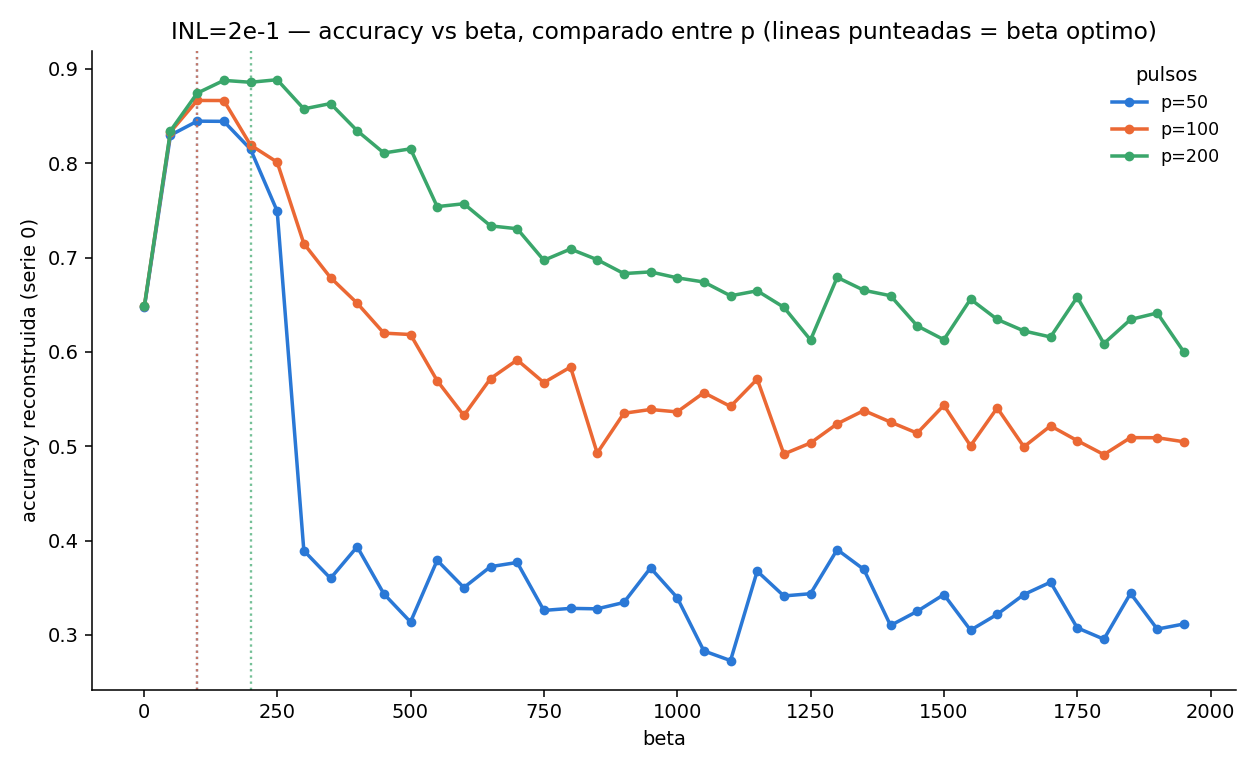
\includegraphics[width=0.85\textwidth]{accuracy_vs_beta_comparado.png}
\caption{Accuracy reconstruida vs $\beta$, las tres curvas superpuestas. Las
líneas punteadas verticales marcan el $\beta$ óptimo de cada una.}
\end{figure}

Las tres curvas suben de forma casi idéntica hasta su $\beta$ óptimo
(arrancan en $\sim$65\,\% en $\beta{=}1$ y llegan a 84--89\,\% en
$\beta\approx100$--200). La diferencia grande aparece \textbf{después} del
óptimo:

\begin{itemize}
\item \textbf{$p=50$}: colapso abrupto tipo acantilado. Entre $\beta{=}200$
  y $\beta{=}300$ la accuracy cae de 81.5\,\% a 38.9\,\%, y después queda
  oscilando sin tendencia entre 27\,\% y 39\,\% hasta $\beta{=}1950$ — un
  régimen básicamente roto.
\item \textbf{$p=100$}: caída más gradual (81.9\,\%$\to$71.5\,\%$\to$
  meseta ruidosa de 50--58\,\% desde $\beta\approx900$) — se degrada
  mucho, pero sin el escalón brusco de $p=50$.
\item \textbf{$p=200$}: caída suave y casi monótona, de 88.6\,\% en
  $\beta{=}200$ a $\sim$60\,\% en $\beta{=}1950$, sin ningún salto abrupto
  — la más robusta a pasarse de $\beta$.
\end{itemize}

O sea: \textbf{a mayor cantidad de pulsos (curva P/D más fina), la red se
vuelve más tolerante a un $\beta$ excesivo}. El mismo patrón aparece en la
calibración: el ECE de $p{=}50$ da un salto brusco justo después del
acantilado (0.044$\to$0.258 entre $\beta{=}250$ y 300), mientras que en
$p{=}100$ y $p{=}200$ el ECE post-óptimo sube de forma progresiva, sin
escalón.

\section{Ejemplo detallado: $p=50$ (la curva con el acantilado más marcado)}

\begin{figure}[htb]
\centering
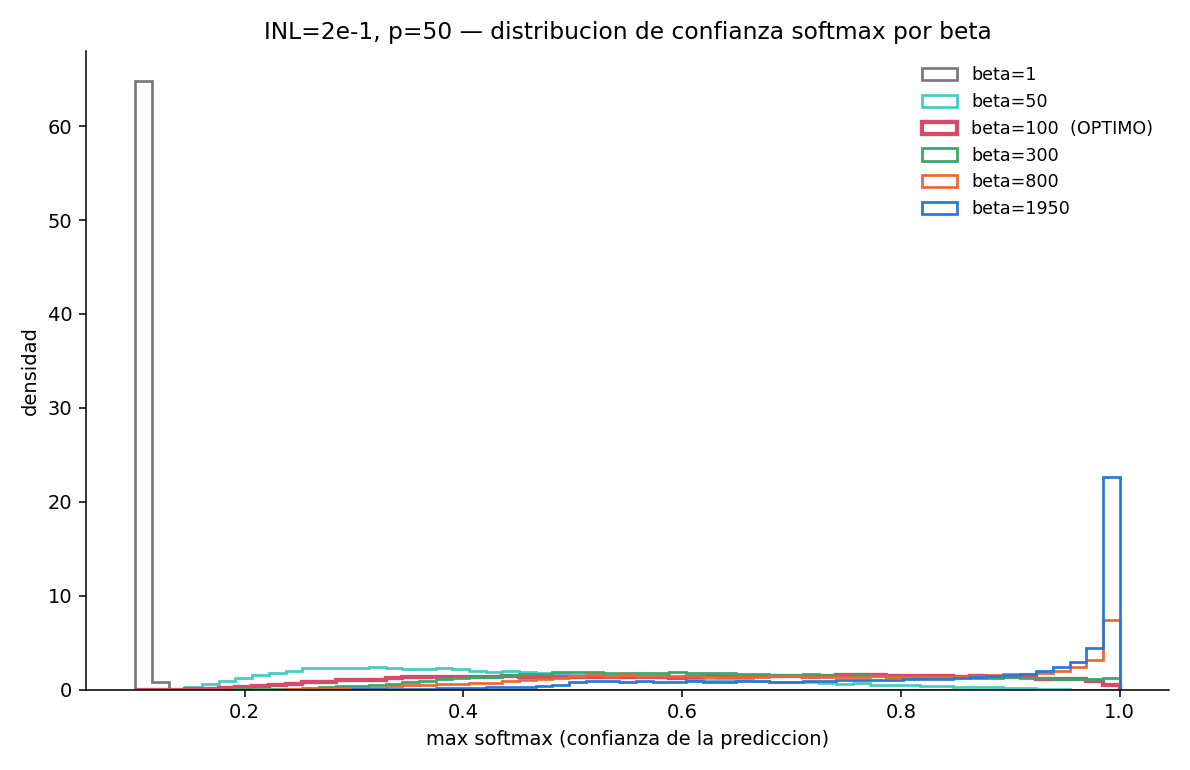
\includegraphics[width=0.8\textwidth]{../analisis_distribucion_softmax_INL_2e-1_p_50/histogramas_maxprob.png}
\caption{Distribución de confianza softmax (max-prob) por $\beta$, $p=50$.
En $\beta$ chico el softmax es casi uniforme (masa pegada a 0.1); en el
óptimo ($\beta{=}100$) ya se separó del uniforme pero sin saturar; en
$\beta$ grande se concentra fuertemente cerca de 1 pese a que la accuracy
real ya colapsó.}
\end{figure}

\begin{figure}[htb]
\centering
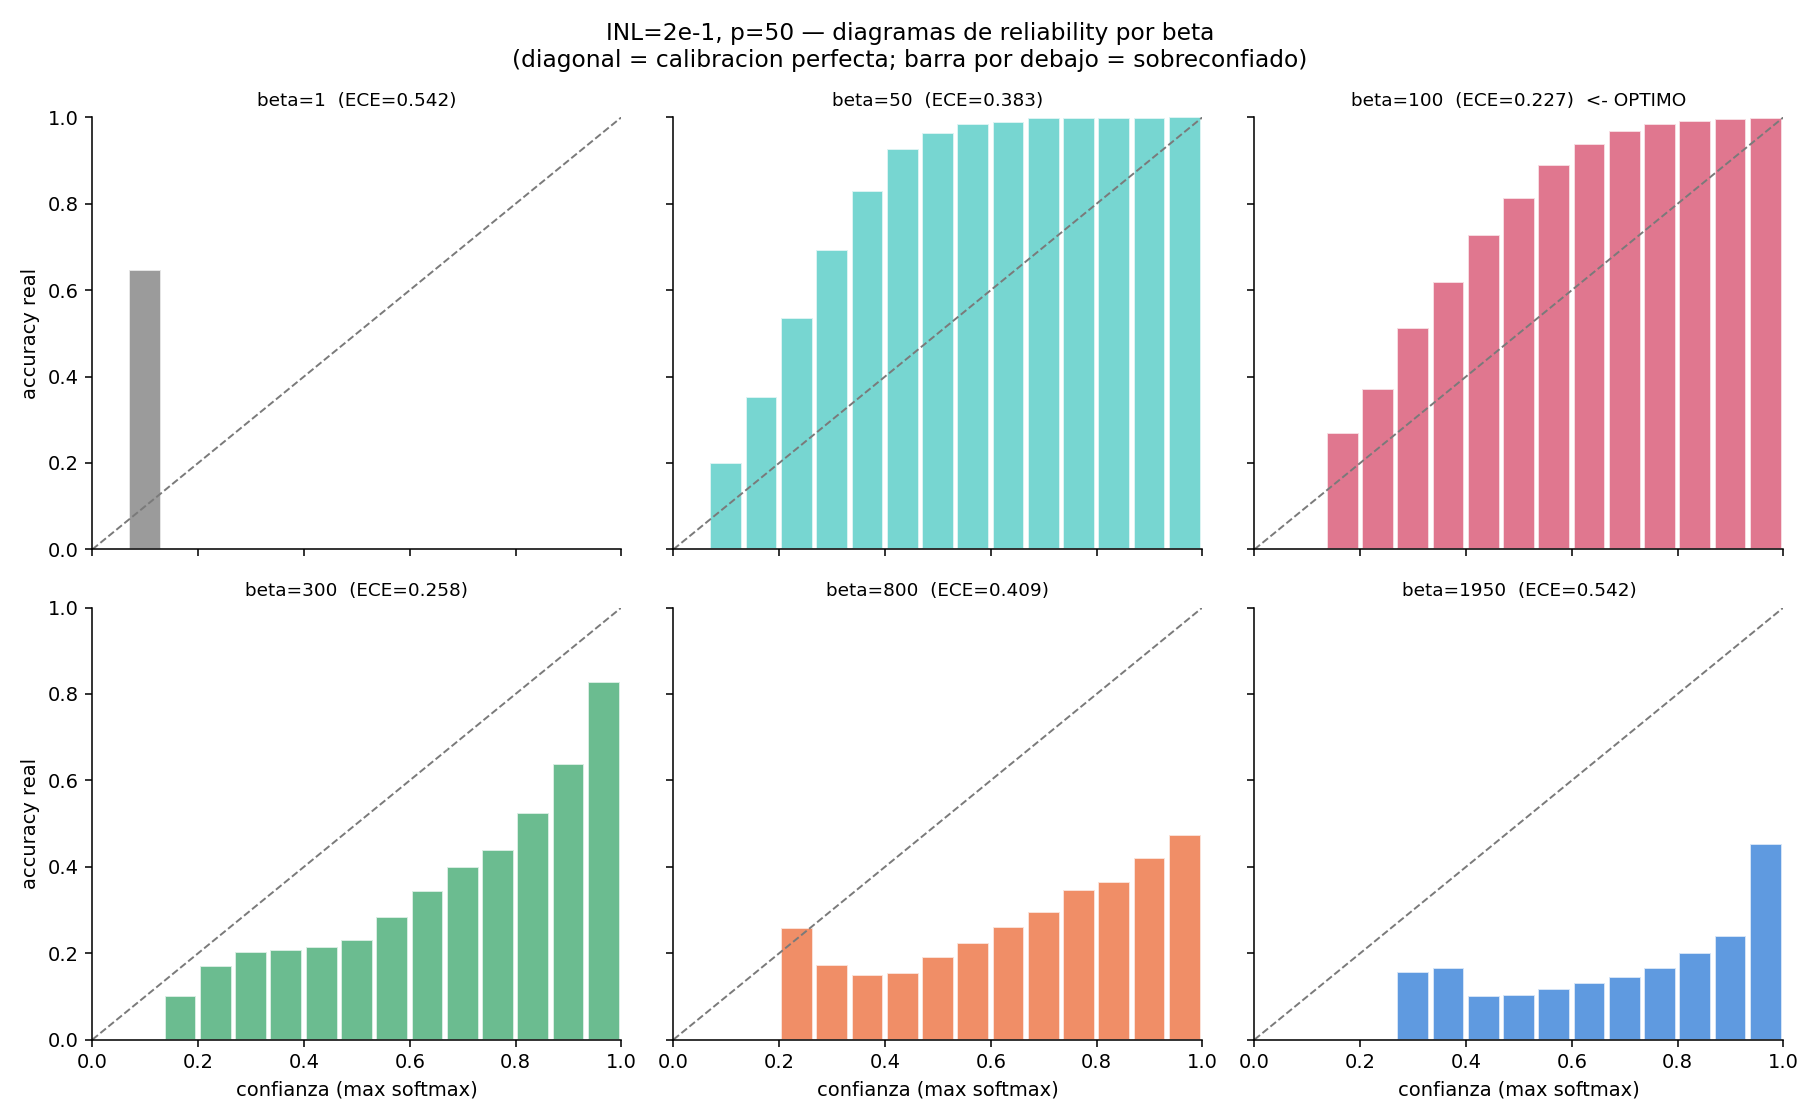
\includegraphics[width=0.85\textwidth]{../analisis_distribucion_softmax_INL_2e-1_p_50/diagramas_reliability.png}
\caption{Diagramas de \emph{reliability} por $\beta$, $p=50$. $\beta$ chico:
subconfiado (barras sobre la diagonal). $\beta$ óptimo: el más cercano a la
diagonal en confianzas altas. $\beta$ grande: sobreconfiado (barras muy por
debajo de la diagonal).}
\end{figure}

Las figuras equivalentes para $p=100$ y $p=200$ (mismo patrón cualitativo,
degradación post-óptimo más suave) están en sus respectivas carpetas
(\texttt{analisis\_distribucion\_softmax\_INL\_2e-1\_p\_100/} y \texttt{..\_p\_200/}).

\section{Lo que SÍ parece común: el desvío estándar de los logits en el óptimo}

\begin{figure}[htb]
\centering
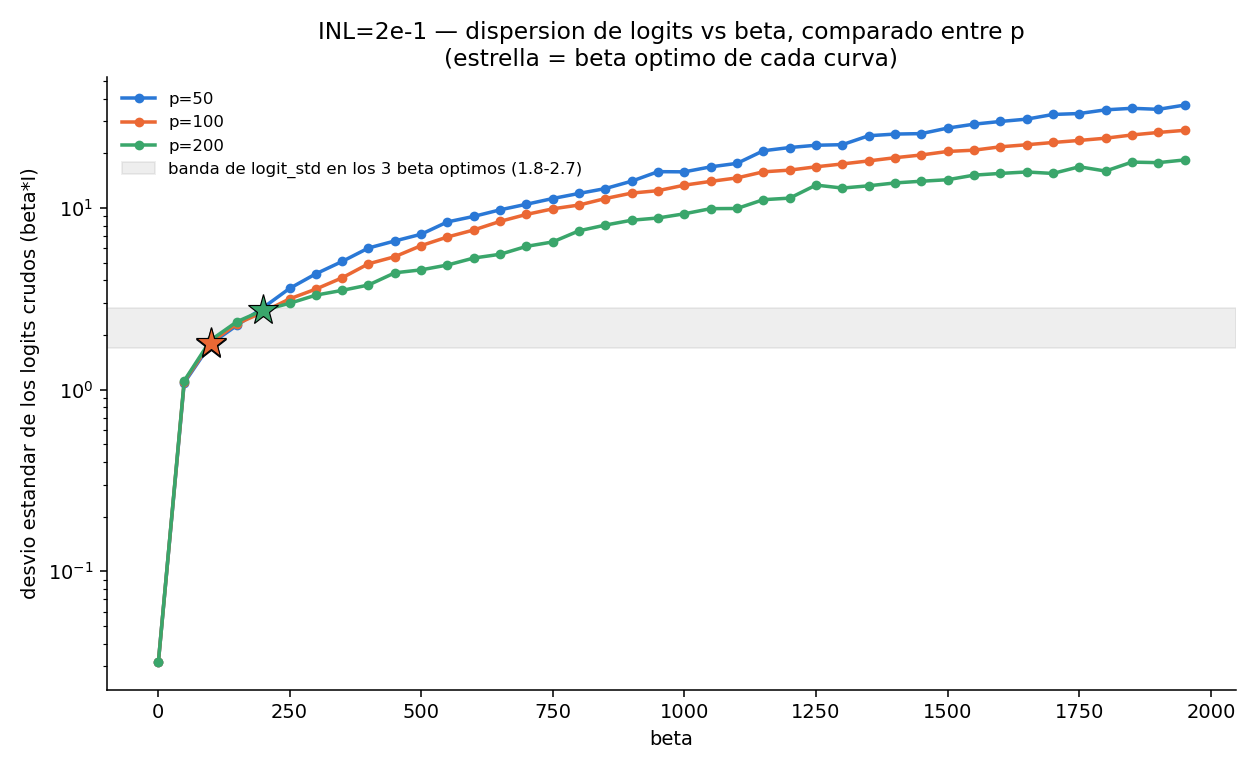
\includegraphics[width=0.85\textwidth]{logit_std_vs_beta_comparado.png}
\caption{Desvío estándar de los logits crudos ($\beta\cdot I$) vs $\beta$,
escala log en $y$. Las estrellas marcan el $\beta$ óptimo de cada curva; la
banda gris marca el rango de \texttt{logit\_std} en esos tres óptimos
(1.8--2.7).}
\end{figure}

\begin{table}[htb]
\centering
\begin{tabular}{@{}rrrrrrrrr@{}}
\toprule
$p$ & $\beta^*$ & accuracy & conf.\ media & entropía & ECE & brecha conf.\ & \textbf{logit std} & frac.\ saturada \\
\midrule
50  & 100 & 0.8446 & 0.617 & 1.213 & 0.227 & 0.269 & \textbf{1.78} & 0.000 \\
100 & 100 & 0.8665 & 0.634 & 1.170 & 0.232 & 0.282 & \textbf{1.82} & 0.000 \\
200 & 200 & 0.8858 & 0.744 & 0.821 & 0.142 & 0.307 & \textbf{2.74} & 0.001 \\
\bottomrule
\end{tabular}
\caption{Métricas en el $\beta$ óptimo de cada curva. Tabla completa:
\texttt{comparacion\_en\_beta\_optimo.csv}.}
\end{table}

$p{=}50$ y $p{=}100$ tienen el \emph{mismo} $\beta$ óptimo (100) y dan un
\texttt{logit\_std} casi idéntico (1.78 vs 1.82 — 2\,\% de diferencia) pese
a tener curvas P/D de distinta resolución. $p{=}200$ tiene $\beta$ óptimo
distinto (200, el doble) y da \texttt{logit\_std}=2.74 — más alto, pero del
mismo orden de magnitud, lejos de los valores de saturación
($\texttt{logit\_std}\gtrsim10$) que aparecen en las tres curvas bien
pasado el óptimo. En las tres, el tramo ``sano'' corresponde a
\texttt{logit\_std} en el rango aproximado \textbf{1.8--3.6}.

Esto es coherente con la lógica de $\beta_{\text{óptimo}}\sim\kappa/\sigma_I$
de \texttt{validacion\_formula\_beta\_optimo/}: si $\kappa\sim O(1)$ es
aproximadamente independiente de $p$, el $\beta$ que hace que
$\sigma_I\cdot\beta$ (el \texttt{logit\_std} de la tabla) caiga en ese
rango angosto es, precisamente, el $\beta$ óptimo — con la salvedad de que
en los datos reales esa cantidad no es una constante perfecta sino que
crece levemente con $p$ (1.78 $\to$ 1.82 $\to$ 2.74).

También son comunes, cualitativamente: la forma en U del ECE vs $\beta$
(mínimo un poco \emph{después} del $\beta$ óptimo, no exactamente en él), y
que la separación de confianza correctos/incorrectos alcance su pico muy
cerca del $\beta$ óptimo en las tres curvas.

\section{Interpretación}

Para \texttt{INL=2e-1} (curva P/D muy no lineal), el $\beta$ óptimo de cada
$p$ cae siempre en la zona de la grilla donde (1) el entrenamiento todavía
converge de forma estable —cuya severidad de ruptura posterior SÍ depende
mucho de $p$— y (2) el desvío estándar de los logits está en un rango
angosto de orden 1--3, prácticamente el mismo entre $p{=}50$ y $p{=}100$ y
solo moderadamente más alto en $p{=}200$. El ``qué tiene de particular''
no está en una propiedad exacta del softmax en sí (ni ECE, ni confianza,
ni entropía tocan su propio óptimo justo en $\beta^*$), sino en que
$\beta^*$ es el $\beta$ más grande que todavía mantiene la dispersión de
los logits dentro de ese rango angosto — más allá de él, la dinámica de
entrenamiento ($\beta$ multiplica también el gradiente) se degrada, a
velocidad muy distinta según $p$.

\section{Próximos pasos (planteados en la primera versión de este reporte)}

Falta repetir este análisis para los \texttt{INL} más chicos (curvas P/D
casi lineales, donde \texttt{accuracy\_vs\_beta\_INL\_*.png} ya sugiere
picos mucho más suaves, sin acantilado) para ver si el rango de
\texttt{logit\_std} en el óptimo se mantiene parecido, y si el
``acantilado de estabilidad'' es propio de curvas P/D muy no lineales
(\texttt{INL} grande) o aparece también, más atenuado, en curvas casi
lineales. \textbf{Esto es exactamente lo que se responde en la
Sección~\ref{sec:ampliacion}}, repitiendo el análisis para
\texttt{INL=1e-2} (curva casi lineal) con los mismos $p=50/100/200$.

\section{Archivos generados (Secciones 1--6, sobre INL=2e-1)}

\begin{itemize}
\item \texttt{comparar\_p.py}, \texttt{comparacion\_en\_beta\_optimo.csv},
  \texttt{accuracy\_vs\_beta\_comparado.png}, \texttt{logit\_std\_vs\_beta\_comparado.png}
  (esta carpeta).
\item Por cada $p$ (\texttt{analisis\_distribucion\_softmax\_INL\_2e-1\_p\_\{50,100,200\}/}):
  \texttt{analizar\_distribucion\_softmax.py}, \texttt{resumen\_por\_beta.csv},
  \texttt{distribuciones\_representativas.npz}, y 6 figuras cada una
  (accuracy, confianza/entropía, calibración, histogramas de confianza y
  de logits, diagramas de reliability).
\end{itemize}

\section{Ampliación: ¿es esto propio de INL=2e-1, o aparece también en curvas casi lineales?}
\label{sec:ampliacion}

Se repitió exactamente el mismo análisis (mismo método, misma serie~0,
misma última época) para \texttt{INL=1e-2} —una curva P/D casi lineal, dos
órdenes de magnitud menos no lineal que \texttt{2e-1}— con los mismos
$p=50/100/200$. Sanity check igual de ajustado: diferencia máxima
$1.7\times10^{-5}$ (p=50), $1.7\times10^{-5}$ (p=100) y $9.4\times10^{-8}$
(p=200) entre accuracy reconstruida y guardada. $\beta$ óptimo empírico:
$p{=}50\rightarrow\beta^*{=}250$ (89.47\,\%), $p{=}100\rightarrow\beta^*{=}350$
(90.91\,\%), $p{=}200\rightarrow\beta^*{=}750$ (91.63\,\%).

Scripts: \texttt{analisis\_distribucion\_softmax\_INL\_1e-2\_p\_\{50,100,200\}/analizar\_distribucion\_softmax.py}
y \texttt{comparar\_INL.py} (esta sección, solo lee los 6
\texttt{resumen\_por\_beta.csv} ya generados).

\subsection{Respuesta (a): el acantilado SÍ es propio de INL grande (muy no lineal)}

\begin{figure}[htb]
\centering
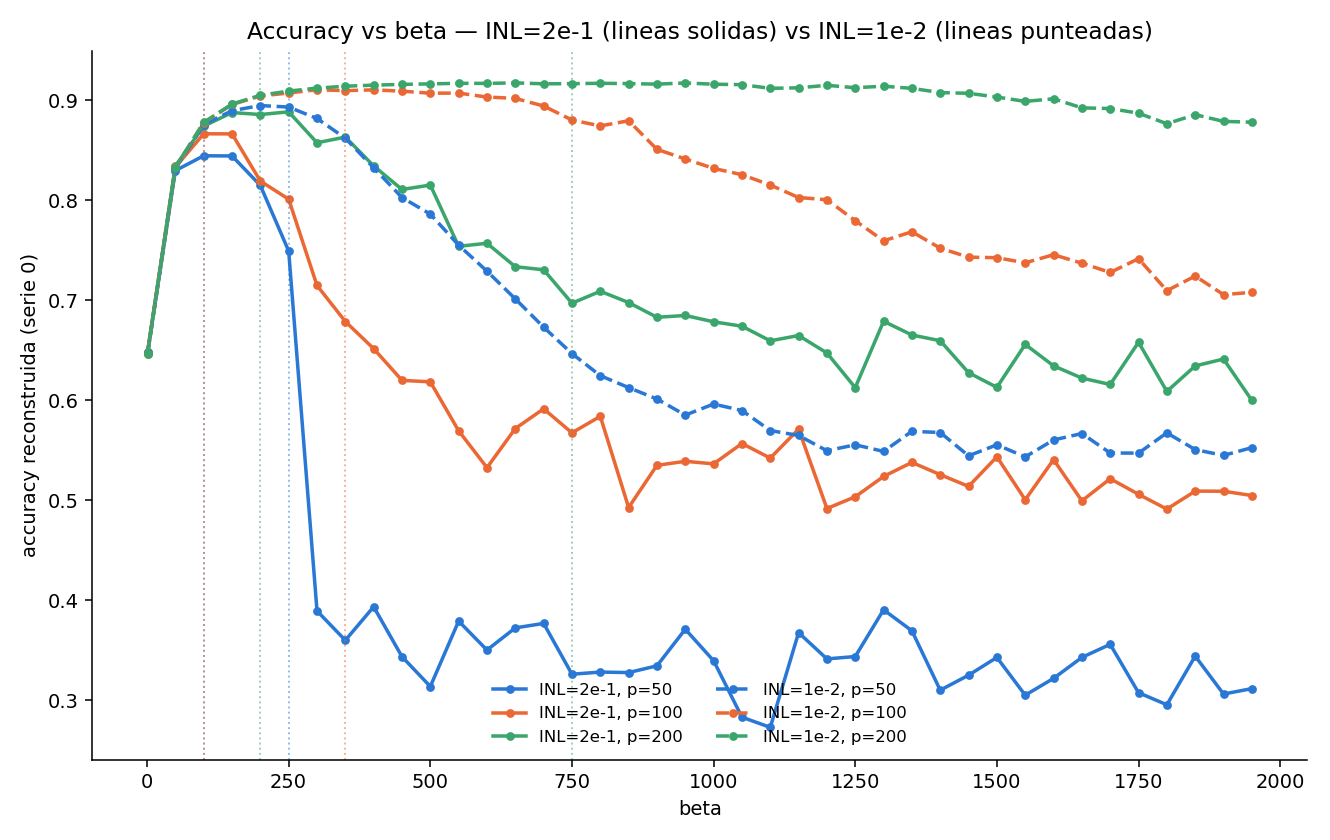
\includegraphics[width=0.9\textwidth]{accuracy_vs_beta_comparado_INL_y_p.png}
\caption{Accuracy vs $\beta$: \texttt{INL=2e-1} (líneas sólidas) vs
\texttt{INL=1e-2} (líneas punteadas), para $p=50,100,200$.}
\end{figure}

La diferencia es enorme y confirma la sospecha de la
Sección~\ref{sec:ampliacion}:

\begin{itemize}
\item \textbf{\texttt{INL=1e-2}, $p=50$}: baja de forma \emph{suave}, sin
  ningún escalón —de 89.3\,\% en $\beta^*{=}250$ a $\sim$55\,\% recién en
  $\beta{=}1950$— mucho más gradual que su contraparte \texttt{INL=2e-1},
  $p=50$, que colapsaba a 30--39\,\% ya en $\beta{=}300$.
\item \textbf{\texttt{INL=1e-2}, $p=100$}: se mantiene por encima de
  90\,\% hasta $\beta\approx650$, y baja gradualmente hasta $\sim$70\,\%
  en $\beta{=}1950$ —sin ningún salto abrupto.
\item \textbf{\texttt{INL=1e-2}, $p=200$}: prácticamente \textbf{una
  meseta}. Se mantiene entre 90.3\,\% y 91.7\,\% desde $\beta{=}200$ hasta
  $\beta\approx1400$, y termina en 87.8\,\% en $\beta{=}1950$ —la accuracy
  casi no se resiente en todo el rango de la grilla. Es, con diferencia,
  la curva más robusta de las 6 analizadas hasta ahora.
\end{itemize}

O sea: \textbf{el ``acantilado de estabilidad'' no es un fenómeno general
del sistema —es específico de curvas P/D muy no lineales (\texttt{INL}
grande)}. Con \texttt{INL} chico (curva casi lineal), aumentar $\beta$
mucho más allá del óptimo degrada la accuracy de forma suave y acotada, en
vez de romper el entrenamiento.

\subsection{Respuesta (b): el \texttt{logit\_std} en el óptimo NO es universal —depende del INL}

\begin{figure}[htb]
\centering
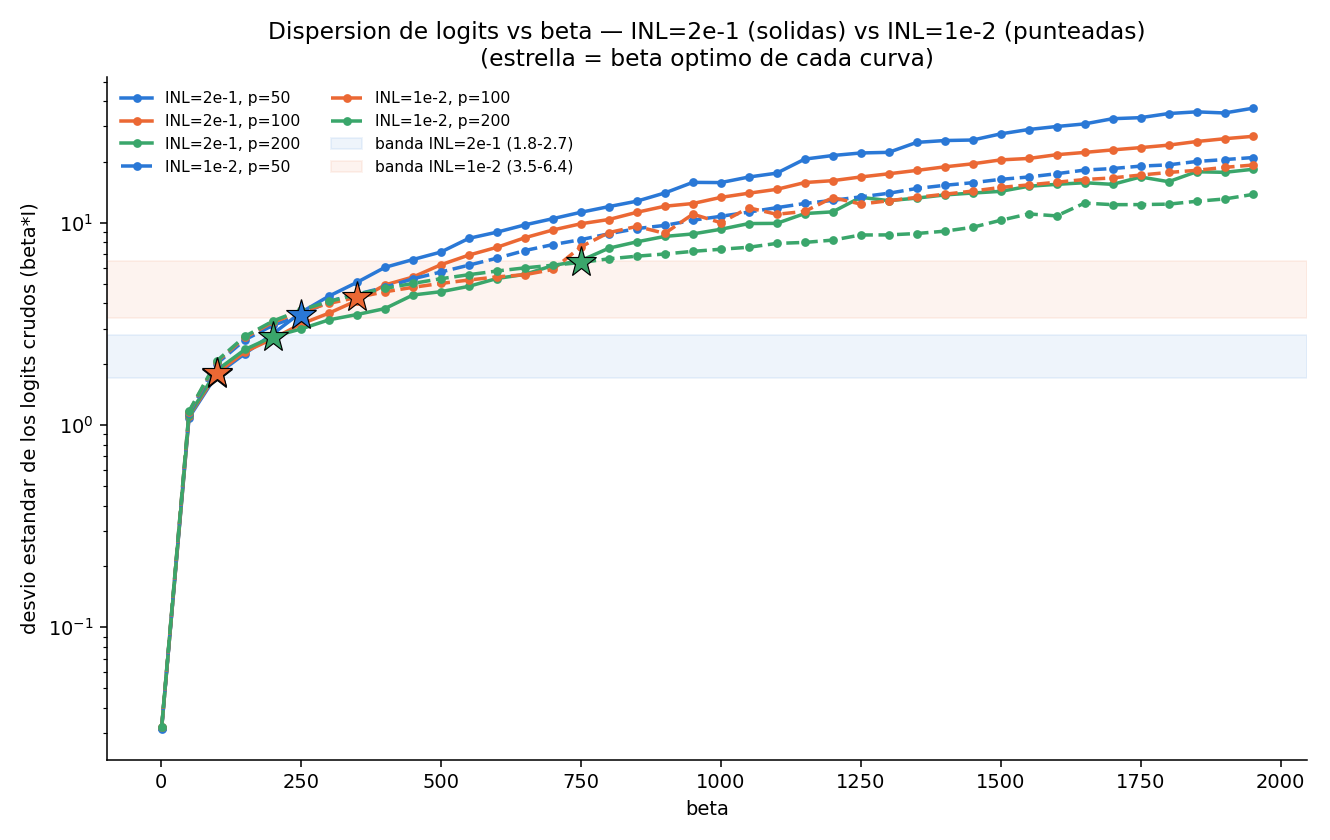
\includegraphics[width=0.9\textwidth]{logit_std_vs_beta_comparado_INL_y_p.png}
\caption{Desvío estándar de los logits crudos vs $\beta$ (escala log),
\texttt{INL=2e-1} (sólidas) vs \texttt{INL=1e-2} (punteadas). Las bandas
sombreadas marcan el rango de \texttt{logit\_std} en los 3 $\beta$ óptimos
de cada INL: no se tocan entre sí.}
\end{figure}

\begin{table}[htb]
\centering
\begin{tabular}{@{}rrrrrrr@{}}
\toprule
INL & $p$ & $\beta^*$ & accuracy & ECE & \textbf{logit std} & frac.\ saturada \\
\midrule
2e-1 & 50  & 100 & 0.8446 & 0.227 & \textbf{1.78} & 0.000 \\
2e-1 & 100 & 100 & 0.8665 & 0.232 & \textbf{1.82} & 0.000 \\
2e-1 & 200 & 200 & 0.8858 & 0.142 & \textbf{2.74} & 0.001 \\
1e-2 & 50  & 250 & 0.8932 & 0.085 & \textbf{3.49} & 0.014 \\
1e-2 & 100 & 350 & 0.9096 & 0.059 & \textbf{4.28} & 0.032 \\
1e-2 & 200 & 750 & 0.9166 & 0.031 & \textbf{6.37} & 0.078 \\
\bottomrule
\end{tabular}
\caption{Métricas en el $\beta$ óptimo, INL x $p$. Tabla completa:
\texttt{comparacion\_en\_beta\_optimo\_INL\_y\_p.csv}.}
\end{table}

La hipótesis de la Sección~4 (banda universal
$\texttt{logit\_std}\approx1.8$--$2.7$) \textbf{no se sostiene entre INL
distintos}: para \texttt{INL=1e-2} el \texttt{logit\_std} en el óptimo es
2--3 veces más alto (3.5--6.4) que para \texttt{INL=2e-1} (1.8--2.7), y las
dos bandas ni siquiera se tocan en la figura de arriba. Lo que sí se
sostiene, y se refuerza con este segundo INL, es la parte más modesta de
la hipótesis: \textbf{dentro de un mismo INL, el \texttt{logit\_std} en el
$\beta$ óptimo queda en un rango angosto y crece solo levemente con $p$}
(\texttt{INL=2e-1}: $1.78\to1.82\to2.74$; \texttt{INL=1e-2}:
$3.49\to4.28\to6.37$ —mismo orden de crecimiento relativo con $p$ en ambos
casos, $\times1.5$--$1.8$ de $p{=}50$ a $p{=}200$).

También es consistente entre ambos INL que la fracción de softmax saturado
en el propio $\beta$ óptimo, aunque nunca despreciable para
\texttt{INL=1e-2} (1.4--7.8\,\%), se mantiene muy por debajo de los
valores $>$15--20\,\% que aparecen bien pasado el óptimo en ambas curvas.

\subsection{Interpretación revisada}

El resultado de la Sección~4 ($\beta$ óptimo $\approx$ el $\beta$ más
grande que mantiene $\texttt{logit\_std}$ en 1.8--2.7) era, en realidad,
una propiedad de \texttt{INL=2e-1} específicamente, no una constante
universal. La versión corregida:

\begin{itemize}
\item Dentro de una misma curva P/D (mismo \texttt{INL}), el
  \texttt{logit\_std} óptimo es aproximadamente estable entre distintos
  $p$ —la fórmula $\beta_{\text{óptimo}}\sim\kappa/\sigma_I$ con $\kappa$
  fijo parece describir razonablemente bien la variación \emph{con $p$, a
  INL fijo}.
\item Pero $\kappa$ (o el \texttt{logit\_std} óptimo efectivo) \textbf{sí
  depende del INL}: una curva P/D más lineal (INL chico) tolera un
  \texttt{logit\_std} óptimo más alto que una muy no lineal (INL grande).
  Tiene sentido cualitativamente: con INL chico los pesos $G^+-G^-$ están
  más concentrados/uniformes, así que la suma $I=\sum W_{ij}V_j$ es una
  variable más ``bien portada'' (más cerca del régimen gaussiano ideal de
  CLT que asume la fórmula), y tolera un $\beta$ mayor antes de que la
  dinámica de entrenamiento se degrade.
\item La severidad de la degradación post-óptimo (el acantilado) también
  depende fuertemente del INL: brusca y catastrófica en \texttt{INL=2e-1},
  ausente o casi ausente en \texttt{INL=1e-2}.
\end{itemize}

\subsection{Próximos pasos (actualizado)}

\begin{itemize}
\item Confirmar la tendencia con un tercer punto de INL (por ejemplo
  \texttt{1e-4} o \texttt{1e-5}, curvas P/D aún más lineales, ya con data
  disponible en \texttt{data\_beta\_grid\_search\_SP/}) para ver si el
  \texttt{logit\_std} óptimo sigue subiendo al bajar el INL, y si se puede
  ajustar una relación funcional simple $\texttt{logit\_std\_óptimo}(\text{INL})$.
\item Extender la comparación de ``severidad del acantilado'' a los INL de
  la zona de transición (\texttt{7e-2}, \texttt{1e-1}, \texttt{1.3e-1},
  \texttt{1.6e-1}, ver \texttt{train\_job\_INL\_7e-2\_p\_50.sh} y afines
  —datos aún no generados/bajados) para ver en qué punto exacto del rango
  de INL aparece el acantilado.
\end{itemize}

\section{Archivos generados (todo el reporte, actualizado)}

\begin{itemize}
\item Secciones 1--6 (solo \texttt{INL=2e-1}): ver Sección~6.
\item Sección~\ref{sec:ampliacion} (\texttt{INL=1e-2}): carpetas
  \texttt{analisis\_distribucion\_softmax\_INL\_1e-2\_p\_\{50,100,200\}/}
  (mismo contenido que sus análogas de \texttt{INL=2e-1}), y en esta
  carpeta: \texttt{comparar\_INL.py}, \texttt{comparacion\_en\_beta\_optimo\_INL\_y\_p.csv},
  \texttt{accuracy\_vs\_beta\_comparado\_INL\_y\_p.png},
  \texttt{logit\_std\_vs\_beta\_comparado\_INL\_y\_p.png}.
\item \texttt{reporte\_distribucion\_softmax\_INL\_2e-1.md} — versión
  Markdown de este mismo reporte (Secciones 1--8).
\end{itemize}

\end{document}
